\documentclass{standalone}
\usepackage{tikz}
\usetikzlibrary{patterns, positioning}
\usepackage[sfdefault]{ClearSans} %% option 'sfdefault' activates Clear Sans as the default text font
\usepackage[T1]{fontenc}

\begin{document}
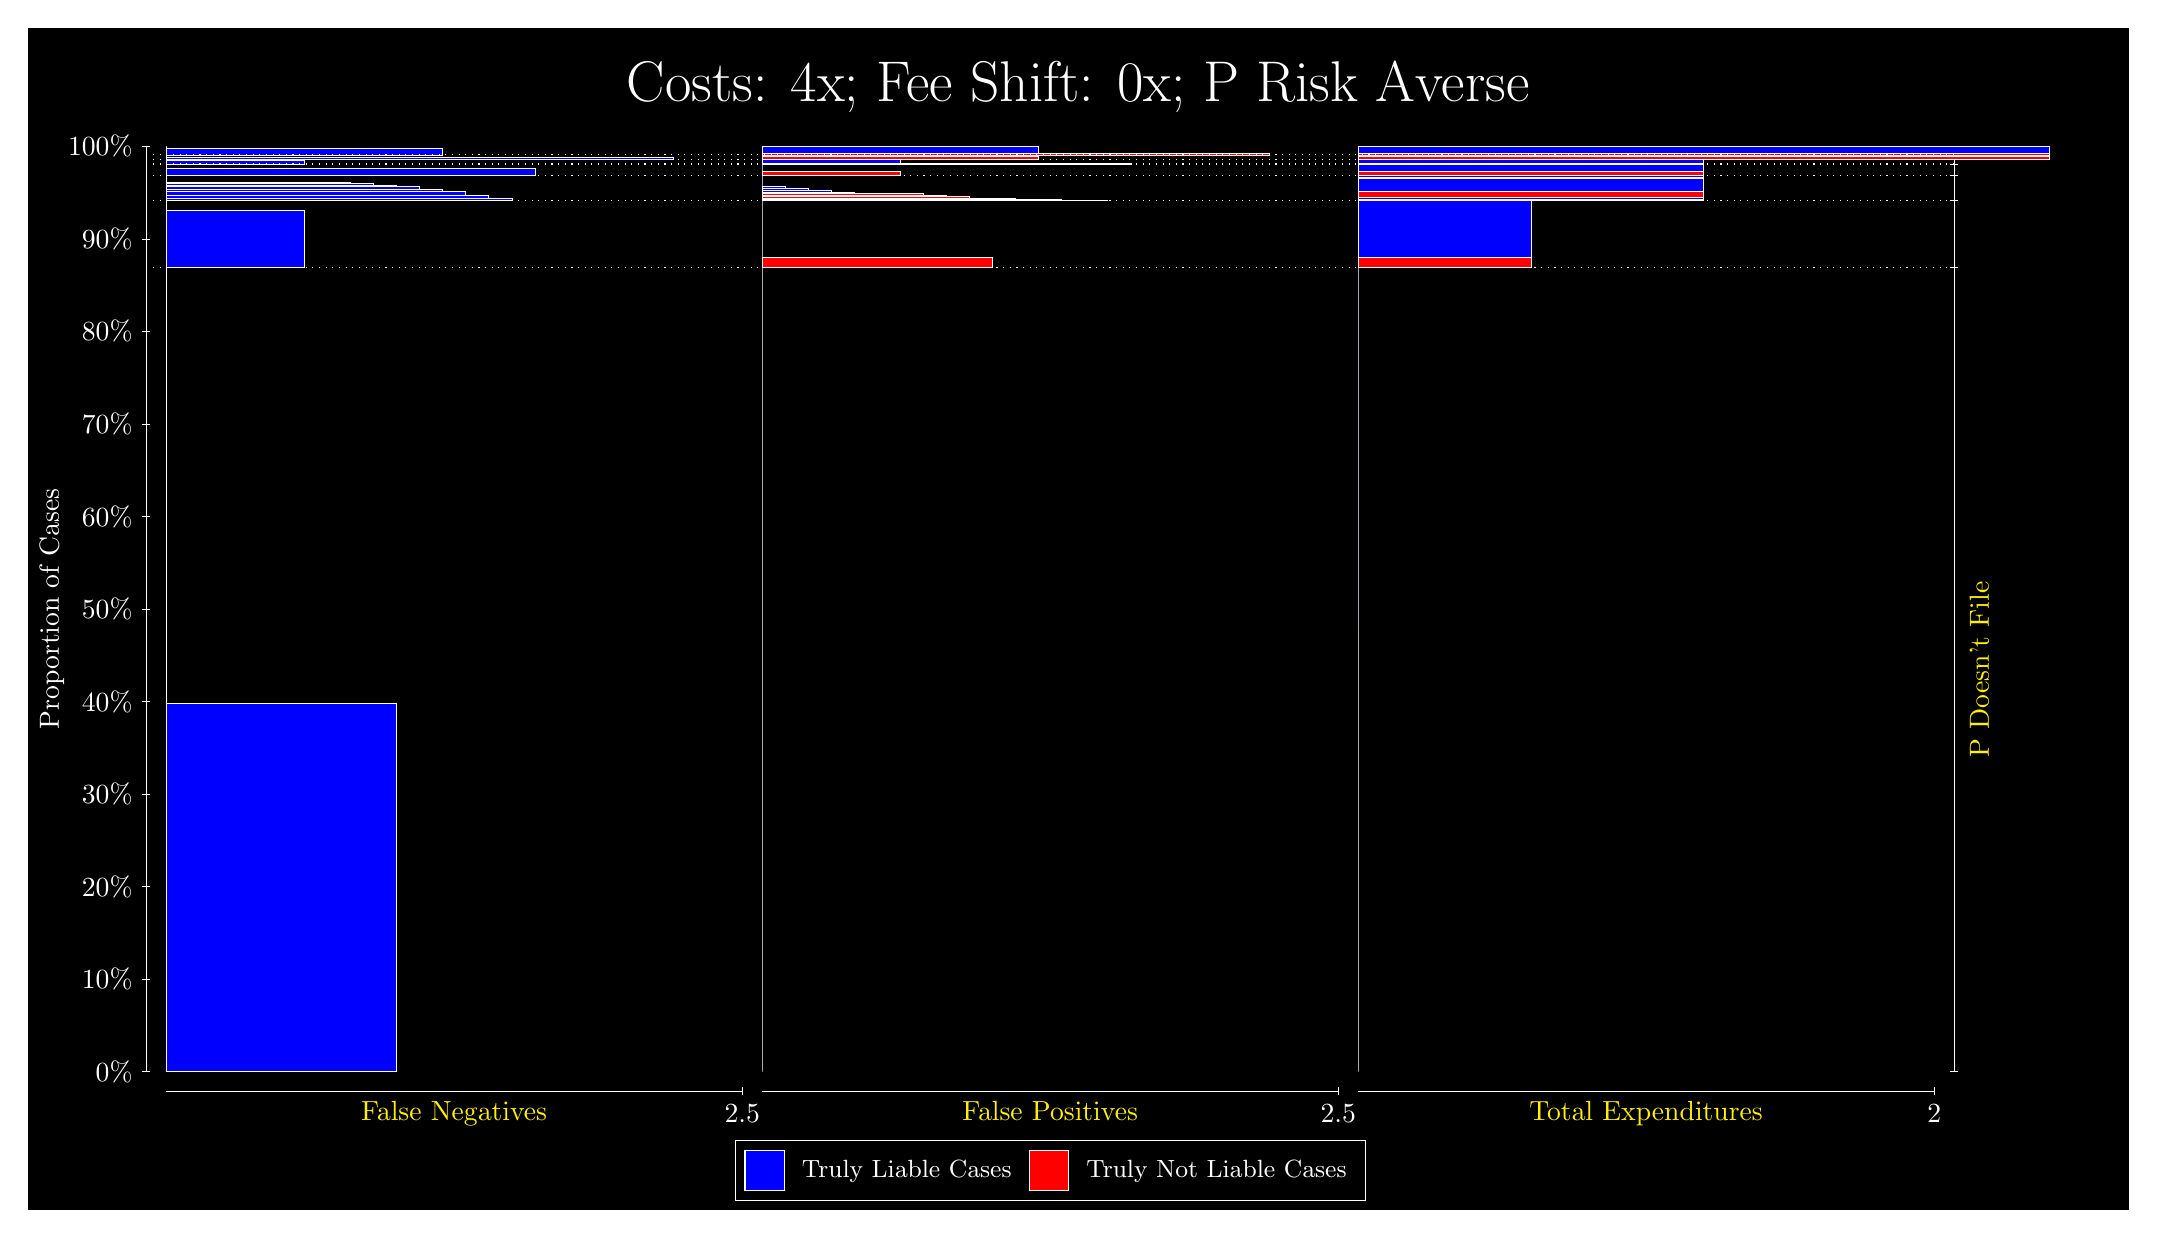
\begin{tikzpicture}
\draw[fill=black] (0,0) rectangle (26.667,15);
\draw[text=white] (0,13.5) rectangle (26.667,15) node[midway] {\huge Costs: 4x; Fee Shift: 0x; P Risk Averse};
\draw[white, very thin] (1.5,1.75) -- (1.5,13.5);
\node[rotate=90, text=white, anchor=center] at (0.3, 7.625) {Proportion of Cases};
\draw[white, very thin] (1.45,1.75) -- (1.55,1.75);
\node[text=white, anchor=east] at (1.45, 1.75) {0\%};
\draw[white, very thin] (1.45,2.925) -- (1.55,2.925);
\node[text=white, anchor=east] at (1.45, 2.925) {10\%};
\draw[white, very thin] (1.45,4.1) -- (1.55,4.1);
\node[text=white, anchor=east] at (1.45, 4.1) {20\%};
\draw[white, very thin] (1.45,5.275) -- (1.55,5.275);
\node[text=white, anchor=east] at (1.45, 5.275) {30\%};
\draw[white, very thin] (1.45,6.45) -- (1.55,6.45);
\node[text=white, anchor=east] at (1.45, 6.45) {40\%};
\draw[white, very thin] (1.45,7.625) -- (1.55,7.625);
\node[text=white, anchor=east] at (1.45, 7.625) {50\%};
\draw[white, very thin] (1.45,8.8) -- (1.55,8.8);
\node[text=white, anchor=east] at (1.45, 8.8) {60\%};
\draw[white, very thin] (1.45,9.975) -- (1.55,9.975);
\node[text=white, anchor=east] at (1.45, 9.975) {70\%};
\draw[white, very thin] (1.45,11.15) -- (1.55,11.15);
\node[text=white, anchor=east] at (1.45, 11.15) {80\%};
\draw[white, very thin] (1.45,12.325) -- (1.55,12.325);
\node[text=white, anchor=east] at (1.45, 12.325) {90\%};
\draw[white, very thin] (1.45,13.5) -- (1.55,13.5);
\node[text=white, anchor=east] at (1.45, 13.5) {100\%};

\draw[white, very thin] (24.457,1.75) -- (24.457,13.5);
\draw[white, very thin] (24.407,1.75) -- (24.507,1.75);
\node[anchor=west] at (24.407, 1.75) {};
\draw[white, very thin] (24.407,11.965) -- (24.507,11.965);
\node[anchor=west] at (24.407, 11.965) {};
\draw[white, very thin] (24.407,12.813) -- (24.507,12.813);
\node[anchor=west] at (24.407, 12.813) {};
\draw[white, very thin] (24.407,13.135) -- (24.507,13.135);
\node[anchor=west] at (24.407, 13.135) {};
\draw[white, very thin] (24.407,13.276) -- (24.507,13.276);
\node[anchor=west] at (24.407, 13.276) {};
\draw[white, very thin] (24.407,13.334) -- (24.507,13.334);
\node[anchor=west] at (24.407, 13.334) {};
\draw[white, very thin] (24.407,13.392) -- (24.507,13.392);
\node[anchor=west] at (24.407, 13.392) {};
\draw[white, very thin] (24.407,13.5) -- (24.507,13.5);
\node[anchor=west] at (24.407, 13.5) {};

\draw[white, very thin, fill=blue] (1.75,1.75) rectangle (4.6775,6.4226);
\draw[white, very thin, fill=red] (1.75,6.4226) rectangle (1.75,11.965);
\draw[white, very thin, fill=blue] (1.75,11.965) rectangle (3.5065,12.69);
\draw[white, very thin, fill=red] (1.75,12.69) rectangle (1.75,12.813);
\draw[white, very thin, fill=blue] (1.75,12.813) rectangle (6.1413,12.846);
\draw[white, very thin, fill=blue] (1.75,12.846) rectangle (5.8486,12.881);
\draw[white, very thin, fill=blue] (1.75,12.881) rectangle (5.5558,12.928);
\draw[white, very thin, fill=blue] (1.75,12.928) rectangle (5.2631,12.951);
\draw[white, very thin, fill=blue] (1.75,12.951) rectangle (4.9703,12.987);
\draw[white, very thin, fill=blue] (1.75,12.987) rectangle (4.6775,13.009);
\draw[white, very thin, fill=blue] (1.75,13.009) rectangle (4.3848,13.031);
\draw[white, very thin, fill=blue] (1.75,13.031) rectangle (4.092,13.041);
\draw[white, very thin, fill=blue] (1.75,13.041) rectangle (3.7993,13.049);
\draw[white, very thin, fill=red] (1.75,13.049) rectangle (1.75,13.135);
\draw[white, very thin, fill=blue] (1.75,13.135) rectangle (6.4341,13.224);
\draw[white, very thin, fill=red] (1.75,13.224) rectangle (1.75,13.276);
\draw[white, very thin, fill=blue] (1.75,13.276) rectangle (3.5065,13.32);
\draw[white, very thin, fill=red] (1.75,13.32) rectangle (1.75,13.334);
\draw[white, very thin, fill=blue] (1.75,13.334) rectangle (8.1906,13.356);
\draw[white, very thin, fill=red] (1.75,13.356) rectangle (1.75,13.392);
\draw[white, very thin, fill=blue] (1.75,13.392) rectangle (5.2631,13.478);
\draw[white, very thin, fill=red] (1.75,13.478) rectangle (1.75,13.5);
\draw[white, very thin, fill=red] (9.3189,1.75) rectangle (9.3189,7.292);
\draw[white, very thin, fill=blue] (9.3189,7.292) rectangle (9.3189,11.965);
\draw[white, very thin, fill=red] (9.3189,11.965) rectangle (12.246,12.088);
\draw[white, very thin, fill=blue] (9.3189,12.088) rectangle (9.3189,12.813);
\draw[white, very thin, fill=red] (9.3189,12.813) rectangle (13.71,12.815);
\draw[white, very thin, fill=red] (9.3189,12.815) rectangle (13.417,12.818);
\draw[white, very thin, fill=red] (9.3189,12.818) rectangle (13.125,12.823);
\draw[white, very thin, fill=red] (9.3189,12.823) rectangle (12.832,12.829);
\draw[white, very thin, fill=red] (9.3189,12.829) rectangle (12.539,12.837);
\draw[white, very thin, fill=red] (9.3189,12.837) rectangle (12.246,12.843);
\draw[white, very thin, fill=red] (9.3189,12.843) rectangle (11.954,12.861);
\draw[white, very thin, fill=red] (9.3189,12.861) rectangle (11.661,12.876);
\draw[white, very thin, fill=red] (9.3189,12.876) rectangle (11.368,12.9);
\draw[white, very thin, fill=blue] (9.3189,12.9) rectangle (10.783,12.908);
\draw[white, very thin, fill=blue] (9.3189,12.908) rectangle (10.49,12.918);
\draw[white, very thin, fill=blue] (9.3189,12.918) rectangle (10.197,12.94);
\draw[white, very thin, fill=blue] (9.3189,12.94) rectangle (9.9044,12.962);
\draw[white, very thin, fill=blue] (9.3189,12.962) rectangle (9.6116,12.997);
\draw[white, very thin, fill=blue] (9.3189,12.997) rectangle (9.3189,13.135);
\draw[white, very thin, fill=red] (9.3189,13.135) rectangle (11.075,13.186);
\draw[white, very thin, fill=blue] (9.3189,13.186) rectangle (9.3189,13.276);
\draw[white, very thin, fill=red] (9.3189,13.276) rectangle (14.003,13.289);
\draw[white, very thin, fill=blue] (9.3189,13.289) rectangle (11.075,13.334);
\draw[white, very thin, fill=red] (9.3189,13.334) rectangle (12.832,13.371);
\draw[white, very thin, fill=blue] (9.3189,13.371) rectangle (9.9044,13.392);
\draw[white, very thin, fill=red] (9.3189,13.392) rectangle (15.759,13.414);
\draw[white, very thin, fill=blue] (9.3189,13.414) rectangle (12.832,13.5);
\draw[white, very thin, fill=red] (16.888,1.75) rectangle (16.888,7.292);
\draw[white, very thin, fill=blue] (16.888,7.292) rectangle (16.888,11.965);
\draw[white, very thin, fill=red] (16.888,11.965) rectangle (19.083,12.088);
\draw[white, very thin, fill=blue] (16.888,12.088) rectangle (19.083,12.813);
\draw[white, very thin, fill=red] (16.888,12.813) rectangle (21.279,12.822);
\draw[white, very thin, fill=blue] (16.888,12.822) rectangle (21.279,12.858);
\draw[white, very thin, fill=red] (16.888,12.858) rectangle (21.279,12.928);
\draw[white, very thin, fill=blue] (16.888,12.928) rectangle (21.279,13.096);
\draw[white, very thin, fill=red] (16.888,13.096) rectangle (21.279,13.104);
\draw[white, very thin, fill=blue] (16.888,13.104) rectangle (21.279,13.135);
\draw[white, very thin, fill=red] (16.888,13.135) rectangle (21.279,13.186);
\draw[white, very thin, fill=blue] (16.888,13.186) rectangle (21.279,13.276);
\draw[white, very thin, fill=red] (16.888,13.276) rectangle (21.279,13.289);
\draw[white, very thin, fill=blue] (16.888,13.289) rectangle (21.279,13.334);
\draw[white, very thin, fill=red] (16.888,13.334) rectangle (25.67,13.371);
\draw[white, very thin, fill=blue] (16.888,13.371) rectangle (25.67,13.392);
\draw[white, very thin, fill=red] (16.888,13.392) rectangle (25.67,13.414);
\draw[white, very thin, fill=blue] (16.888,13.414) rectangle (25.67,13.5);
\draw[white, dotted] (1.5,11.965) -- (24.457,11.965);
\draw[white, dotted] (1.5,12.813) -- (24.457,12.813);
\draw[white, dotted] (1.5,13.135) -- (24.457,13.135);
\draw[white, dotted] (1.5,13.276) -- (24.457,13.276);
\draw[white, dotted] (1.5,13.334) -- (24.457,13.334);
\draw[white, dotted] (1.5,13.392) -- (24.457,13.392);
\draw[white, very thin] (1.75,1.5) -- (9.0689,1.5);
\node[text=yellow, anchor=north] at (5.4094, 1.5) {False Negatives};
\draw[white, very thin] (9.0689,1.45) -- (9.0689,1.55);
\node[text=white, anchor=north] at (9.0689, 1.45) {2.5};

\draw[white, very thin] (9.3189,1.5) -- (16.638,1.5);
\node[text=yellow, anchor=north] at (12.978, 1.5) {False Positives};
\draw[white, very thin] (16.638,1.45) -- (16.638,1.55);
\node[text=white, anchor=north] at (16.638, 1.45) {2.5};

\draw[white, very thin] (16.888,1.5) -- (24.207,1.5);
\node[text=yellow, anchor=north] at (20.547, 1.5) {Total Expenditures};
\draw[white, very thin] (24.207,1.45) -- (24.207,1.55);
\node[text=white, anchor=north] at (24.207, 1.45) {2};

\node[text=yellow, centered, rotate=90] at (24.777, 6.8573) {P Doesn't File};







\draw (12.978300999999998,1.5) node[draw=none] (baseCoordinate) {};
\begin{scope}[align=center]
        \matrix[scale=0.5, draw=white, below=0.5cm of baseCoordinate, nodes={draw}, column sep=0.1cm]{
            \node[rectangle, draw, minimum width=0.5cm, minimum height=0.5cm, fill=blue] {}; &
            \node[draw=none, font=\small, text=white] (B) {Truly Liable Cases}; &
            \node[rectangle, draw, minimum width=0.5cm, minimum height=0.5cm, fill=red] {}; &
            \node[draw=none, font=\small, text=white] (B) {Truly Not Liable Cases}; \\
            };
\end{scope}

\end{tikzpicture}
\end{document}